\chapter{Grobkonzept und technische Grundlagen}
\label{TechnischeGrundlagen}
Dieses Kapitel beginnt mit dem Grobkonzept des Longboards Commute, um einen Überblick über das Elektroskateboard zu geben. Anschliessend werden die notwendigen technischen Grundlagen für die Hard- und Software erklärt.

\section{Grobkonzept}
\label{Grobkonzept}
Das Projekt Commute von Skatemate kann in drei Grundbereiche unterteilt werden: Die innovative Steuerung, die Motorregelung und die Stromversorgung. \\
In den folgenden Unterkapitel werden diese drei Bereiche und die dazugehörigen Begriffe detaillierter erläutert. Die intuitive Bedienung des Longboards geschieht über eine Fingerbewegung, welche dank des Magic Gloves gemessen werden kann. Der Motor wird mithilfe der feldorientierten Regelung (field oriented controll FOC) angesteuert, mit dieser Regelungstechnik können Wechselgrössen elegant gesteuert werden. Die Stromversorgung verfügt über ein eigens dazu konzipiertes Akkuladegerät. 
\begin{figure}[H]
	\centering
	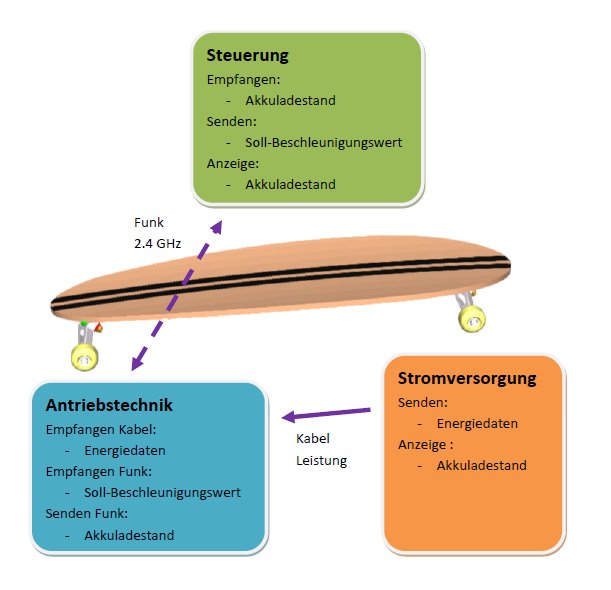
\includegraphics[width=0.8\linewidth, keepaspectratio]{images/Grobkonzept_Blockschaltbild_grob}
	\caption[Blockschaltbild Grobkonzept]{Blockschaltbild Grobkonzept}
	\label{fig:grobkonzeptblockschaltbildgrob}
\end{figure}
Die Abbildung \ref{fig:grobkonzeptblockschaltbildgrob} stellt die Interaktion zwischen den drei Bereichen dar. Die Antriebstechnik ist über ein Kabel mit der Stromversorgung verbunden, die Inputs der Steuerung erhält sie über ein Funknetz. \\
Um eine Übersicht über die enthaltenen Komponenten der drei genannten Bereiche zu erhalten, sind sie im Blockschaltbild der Abbildung \ref{fig:grobkonzeptblockschaltbilddetailliert} dargestellt. \\
Für die Steuerung wird die vom Flex-Sensor gemessene Krümmung des Fingers an der Mikrocontroller weitergeleitet. Dieser Verarbeitet diese in eine Wunschbeschleunigung und leitet sie mithilfe eines Funkmoduls an die Antriebstechnik weiter. Zudem steuert er die Front-LEDs an. Mit Strom versorgt wird der Mikrocontroller und das Funkmodul mithilfe einer Knopfbatterie. \\
Der Mikrocontroller der Antriebstechnik erhält die Wunschbeschleunigung wiederum über ein Funkmodul. Mit der FOC werten daraus die benötigten PWM-Spannungen berechnet. Diese werden durch eine H-Brücke, bestehend aus den Treiber und FETs, am Motor angelegt. Versorgt werden die Treiber und somit der Motor über die Akku-Stromversorgung. \\
Zwischen der Akkuspannung und den Treibern ist ein elektrischer Schalter. Dieser wird über den Mikrocontroller der Stromversorgung gesteuert. Der Mikrocontroller steuert auch den Ladevorgang, also das Balancing. 

\begin{figure}[h]
	\centering
	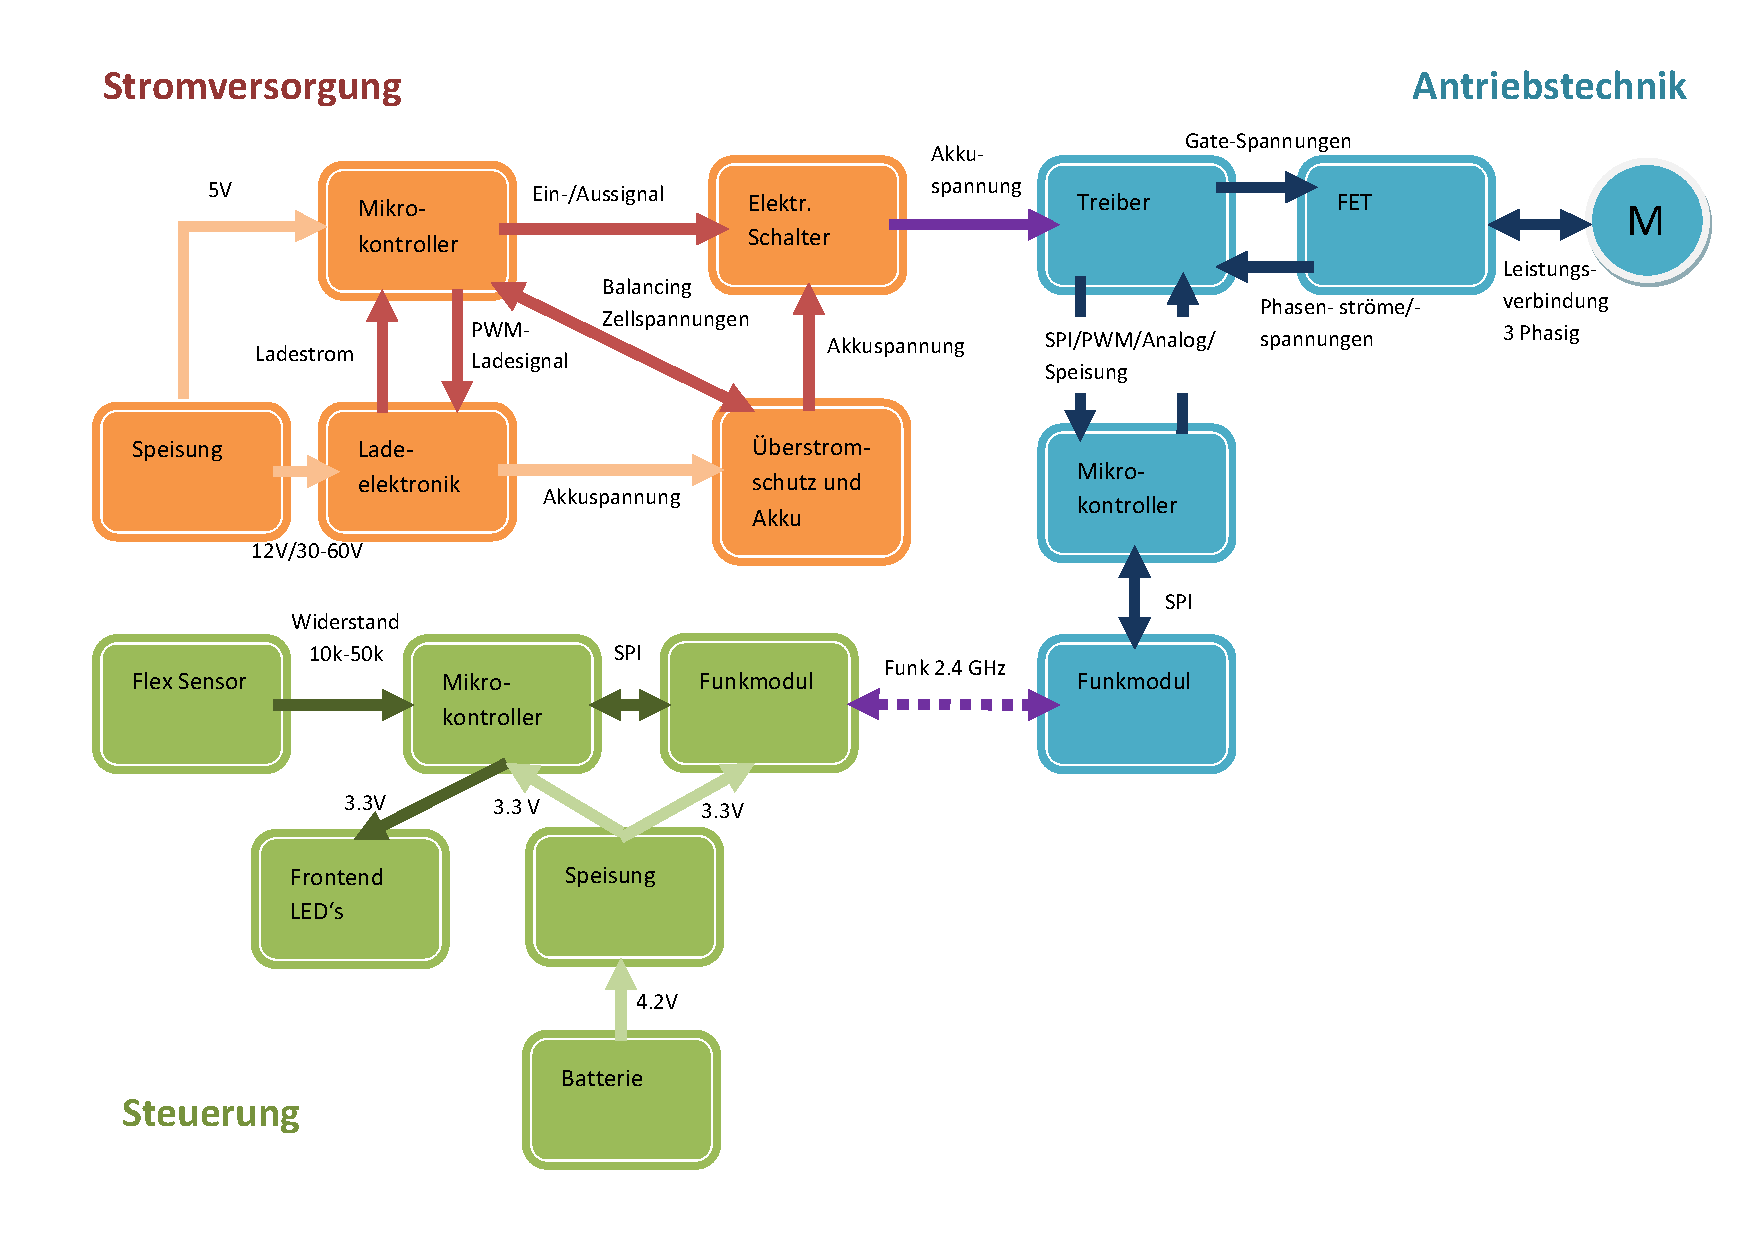
\includegraphics[width=\linewidth]{images/Grobkonzept_Blockschaltbild_detailliert}
	\caption[Detailliertes Blockschaltbild]{Detailliertes Blockschaltbild}
	\label{fig:grobkonzeptblockschaltbilddetailliert}
\end{figure}

\subsection*{Steuerung über den Magic Glove}
Es gibt verschiedene Wege, wie ein elektrisches Longboard gesteuert werden kann. 
Eine Variante ist, Drucksensoren ins Brett einzubauen.
Mit einer Gewichtsverlagerung in oder gegen die Fahrtrichtung wird eine Geschwindigkeitsregulation erreicht. Da auf unebenem Gelände das Gewicht laufend ausbalanciert werden muss, müssten diese Bewegungsimpulse kompensiert werden. Ausserdem können lokal begrenzte Sensoren die Bewegungsfreiheit auf dem Longboard einschränken.
Aus diesen Gründen wurde diese Variante verworfen. \\
Das Team hat sich stattdessen entschieden, die Geschwindigkeit über eine Fingerbewegung zu steuern. Dazu wird ein Handschuh mit integrierten Sensoren entwickelt. Dieses Wearable enthält einen Flex-Sensor, der die Beugung des Zeigefinders misst. Dieser Messvorgang und der Flex-Sensor werden im Kapitel \ref{tGl_FlexSensor} beschrieben. Der Mikrocontroller quantifiziert die mit dem Flex-Sensor gemessene Beugung des Fingers.
Diese Sollbeschleunigung wird anschliessend an die Motoransteuerung übermittelt. Dies geschieht über ein 2.4GHz-Funknetz, dazu ist ein Funkmodul integriert. Die Stromversorgung erfolgt über eine Li-Ion Knopfbatterie LTR2450. In der Abbildung \ref{fig:grobkonzeptblockschaltbilddetailliert} sind die genannten Elemente der Steuerung dargestellt.

\subsection*{Antriebstechnik}
Als Antrieb ist der OX1 2-10 Motor vorgegeben. Dies ist ein Bürstenloser-Gleichstrommotor (brushless DC motor, BLDC-Motor). Er verfügt über keine Hallsensoren, mit denen die Rotorposition gemessen werden könnte. Ein BLDC-Motor ist wie ein permanentmagnetischer Drehstrom-Synchronmotor (PMSM) aufgebaut. Die technischen Hintergründe des Motors werden im Kapitel \ref{tGl_BLDC} gegeben. 
\\
Zur Ansteuerung gibt es grob unterteilt zwei verschiedene Arten, die Kommutierung und die Feldorientierte Regelung \cite{BLDC}. Die Kommutierung wiederum kann auf zwei verschiedene Arten erfolgen, ungesteuert (Blockkommutierung) oder gesteuert (Sinus-Kommutierung). Diese resultierenden drei Ansteuerungsmöglichkeiten sind in der Tabelle \ref{tabMotcontrVarProCon} zur Übersicht dargestellt und nachfolgend etwas genauer erläutert. 
\begin{center}
	\begin{tabularx}{\textwidth}{l|X|X}
		Regelungsart & Vorteile & Nachteile \\ 
		\hline 
		Blockkommutierung & -einfach & -schlechte Effizienz (eine Spule nicht gebraucht) 
		
		-Drehmoment-Rippel \\
		\hline 
		Sinus-Kommutierung & -alle drei Spulen benutzt & -kompliziert
		
		-Anfahren erschwert \\ 
		\hline 
		FOC & -dynamisch 
		
		-effizient 
		
		-durch Trafo einfacher PI-Regler & -Einstieg komplex \\ 
		\hline 
	\end{tabularx} 
	\captionof{table}{Vor- und Nachteile der verschiedenen Regelungsarten}
	\label{tabMotcontrVarProCon}
\end{center}

Bei der ungesteuerten Kommutierung (Blockkommutierung) wird der Motor als Schrittmotor genutzt. Dabei folgt die Rotorposition der Steuerung. Diese Variante ist für ein gleichmässig rollendes Longboard ungeeignet, da der Schrittmotor nicht durchgehend, sondern immer nur schrittweise dreht. \\
Für ein gleichmässiges Drehen muss die Kommutierung also abhängig von der Rotorposition erfolgen (geführte Kommutierung, Sinus-Kommutierung). Dabei reagiert die Steuerung auf die effektive Rotorposition und passt sich dieser an.\todo{(xxx korrekt?} Am einfachsten wäre dies mit Sensoren. Da der Motor jedoch über keine Sensoren verfügt, muss er über eine sensorlos gesteuerte Kommutierung angesteuert werden. Dies funktioniert jedoch nur ab einer Mindestdrehzahl wirklich gut. Zum Anfahren muss der Motor speziell angesteuert werden. \\
Bei der Feldorientierte Regelung  werden die Spannungen zur Steuerung aktiv der Rotorlage angepasst. Dabei kann zwischen sensorgesteuerter und sensorloser Regelung unterschieden werden. Bei der sensorlosen Regelung muss wiederum zum Anfahren eine zusätzliche Ansteuerung erfolgen. Kann die Anfangsposition ausreichend genau geschätzt werden, läuft der Motor auch bei tiefen Geschwindigkeiten gleichmässig, da er genauer geregelt werden kann. Dies entspricht den Anforderungen für das Commute, da ein sanftes Anfahren sehr wichtig ist. Die FOC als auch die Anfahr-Ansteuerung ist im Kapitel \ref{tGl_FOC} erklärt.\\
Ausgeführt wird die FOC auf einem Mikrocontroller. Mittels RF-Modul wird die Sollbeschleunigung empfangen. Eine Halbbrücke mit FET-Treibern (siehe Kapitel \ref{tGl_HBrugg}) setzt  die gewünschte Motorsteuerung um. Zur Übersicht sind diese Elemente im Blockschaltbild Abbildung \ref{fig:grobkonzeptblockschaltbilddetailliert} dargestellt. 

\subsection*{Stromversorgung}
Die Stromversorgung erfolgt über einen LiPo-5200mAh-Akku, dieser ist vorgegeben. Bei einer durchschnittlichen Leistungsaufnahme von 50W des Motors reicht eine Akkuladung ungefähr für zwei Stunden Fahrt. Auch ein externes Ladegerät ist gestellt, doch um dieses zu nutzen, müsste der Akku für jedes Laden vom Longboard gelöst werden. Das ist umständlich und gefährdet die Wetterfestigkeit und Robustheit des Commute. Deshalb wird ein eigener, integrierter Akkulader entwickelt, so dass der Akku nicht mehr herausgelöst werden muss. Da die Entladung im Gebrauch sowieso überwacht werden muss, ist der Lader eine Ergänzung und kein alleinstehendes Element. \\ Kernstück der Stromversorgung ist die Balancerschaltung. Dabei wird der Akku erst mit einem konstanten Strom geladen, bis die Zellspannung erreicht ist. Anschliessend wird mit einer konstanten Spannung geladen, bis der Strom unter 100mA gesunken ist, dann sind die Zellen vollständig geladen. Wie das Balancing genau funktioniert, ist im Kapitel \ref{tGl_Balancing} beschrieben. Anstelle einer eigenen Implementation hätte ein fertiges IC eingekauft werden können. Aus finanziellen Gründen wurde jedoch darauf verzichtet. Wie bereits erwähnt sind die Elemente der Stromversorgung in der Abbildung \ref{fig:grobkonzeptblockschaltbilddetailliert} übersichtlich dargestellt.

\todo{ev: wie viel Strom braucht der Motor? Wie weit reicht eine Akkuladung?
Ich rechne metere Durchschnittliche Leistigsufnahm vo 50W. De akku het 5.3*22.2=118Wh, das heist me chan 2h fahre ohni de akku tüfentlade}


%-----------------------------------------------------------------------------------------------------------------------------------------------------------------------------

\section{Technische Grundlagen}
In den folgenden Unterkapiteln werden die technischen Grundlagen zum Verständnis der Hard- und Software erläutert, so dass deren Funktionsweisen verstanden werden können.  Dazu werden für die Steuerung der Flex-Sensor (Kapitel \ref{tGl_FlexSensor}) und die Funkübertragung (Kapitel \ref{tGl_RF}), für die Stromversorgung das Balancing (Kapitel \ref{tGl_Balancing}) und für die Motoransteuerung der BLDC-Motor (Kapitel \ref{tGl_BLDC}), die FOC (Kapitel \ref{tGl_FOC}) und die Treiber und FETs (H-Brücke, Kapitel \ref{tGl_HBrugg}) erklärt.

\subsection{Flex-Sensor}
\label{tGl_FlexSensor}
Ein Flex-Sensor eignet sich dazu, als analoges elektrisches Bauteil, eine Biegung zu messen. Im Falle dieses Projekts heisst dies, zu erkennen wie fest der Finger des Fahrers gebogen ist. 
Der Sensor ändert je nach Biegung seinen Widerstandswert im Bereich von 13 bis ca. 80k$\Omega$ bei der stärksten Verformung. Das Bauteil selbst besteht aus einem flexiblen PCB mit einer darauf befestigten Schicht von metallischen Partikeln. Wird der Sensor nun gebogen, entfernen sich die Partikel voneinander, wodurch sich der Widerstand vergrössert. Biegt man den Sensor zurück in seine Ausgangsposition, verkleinert sich der Widerstandswert wieder.
\\
Um diesen Widerstand messen zu können, wurde eine Verstärkerschaltung mit Messbrücke aufgebaut (Abbildung \ref{fig:gl_Flex-Sensor}). Der Widerstand der als Flex-Sensor angeschrieben ist, verfügt über einen Wertebereich von 13 bis 80 k$\Omega$. Mit den beiden Widerständen R2 und R3 wird die Untergrenze der messbaren Resistanz festgelegt. Mit R1 wird schliesslich die Skalierung der Brücke festgelegt. Die resultierenden Spannungen zwischen R1 und R2 bzw. zwischen R3 und R4 werden schliesslich durch einen Rail-To-Rail Operationsverstärker so fest verstärkt, dass sie den Spannungsbereich von 0 bis 3.3 Volt ausnutzen. Dadurch kann schliesslich der
angehängte 10bit A/D-Wandler vollständig ausgesteuert werden.
\begin{figure} [H]
	\centering
\subfigure[Funktionsprinzip Flex-Sensor]{
	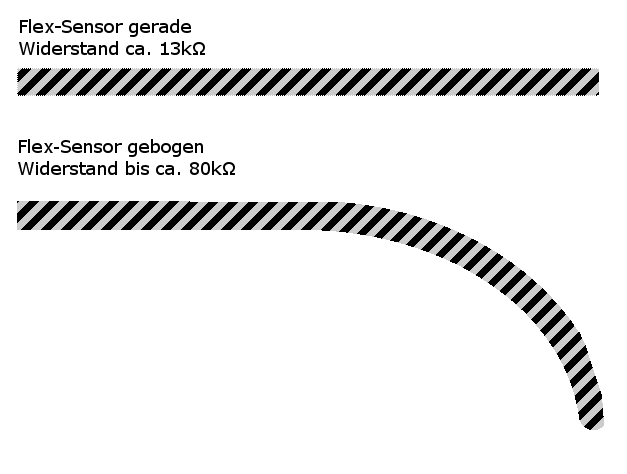
\includegraphics[width=0.45\linewidth]{images/FlexSensor} \label{FlexSensor} 	}
\subfigure[Sinstr][Messbrücke für Flex-Sensor]{ 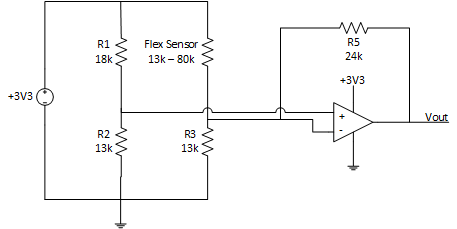
\includegraphics[width=0.5\linewidth]{images/FlexSensor_Messbruecke} \label{FlexSensor_Messbruecke}}
\caption[FlexSensor]{Funktionsprinzip und Ansteuerung für einen Flex-Sensor}
\label{fig:gl_Flex-Sensor}
\end{figure}

\subsection{Balancing}
\label{tGl_Balancing}
Das Board wird durch einen sechs Zellen-LiPo-Akku gespeist. Jede einzelne Zelle hat dabei einen eigenen Innenwiderstand, der sich mit dem Alter verändern kann. Beim Ladevorgang entstehen somit unterschiedliche Spannungen, wodurch die Zellen aus der Balance geraten.
Damit sich einzelne Zellen nicht überladen, während andere leer bleiben, benötigt es einen Balancing-Vorgang um die Differenzen der Zellen auszugleichen. 
Dabei werden bei einer zu grossen Spannungsdifferenz alle Zellen auf die Spannung der niedrigsten Zelle entladen.
Dazu wird die überschüssige Energie über den Transistor und die Widerstände verheizt.

\subsection{BLDC-Motor}
\label{tGl_BLDC}
Für dieses Projekt ist der Motor OX1 2-10 zur Verfügung gestellt worden. Dabei handelt es sich um einen dreiphasigen Brushless-DC-Motor ohne Hallsensoren (Sensoren zur Rotorpositionsermittlung). Die gegebenen technischen Daten sind in der Tabelle \ref{tabBLDCdaten} ersichtlich.
Ein BLDC-Motor ist aufgebaut wie eine permanenterregte Synchronmaschine. Der OX1 2-10 ist als Aussenläufermotor gebaut.
Die Erregung des Motors erfolgt mit 14 Permanentmagneten, er verfügt somit über sieben Polpaaren. Der Stator besteht aus 12 Spulen, also ist jede Phase vier Mal gewickelt. 
In der Abbildung \ref{figAufbauBLDC} ist das Feldverhalten dargestellt.\\

\begin{figure} [H]
%	\centering
\subfigure[Prinzip Aufbau BLDC \cite{ElAntriebe_Babiel}]{
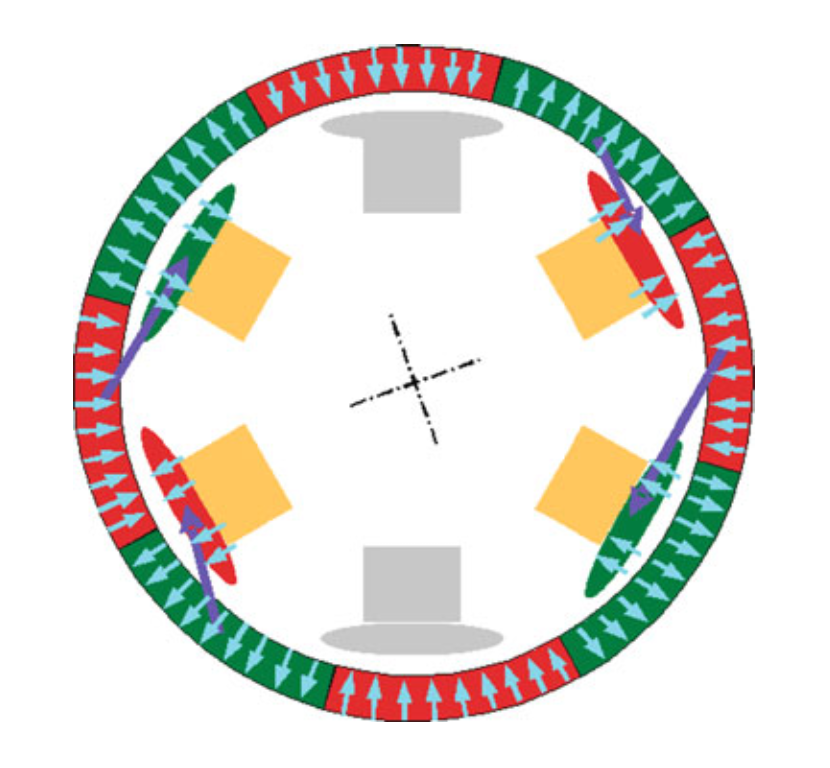
\includegraphics[width=0.45\linewidth]{images/AufbauBLDC} \label{figAufbauBLDC} 	}
\subfigure[Sinusstrom mit PWM-Spannung \cite{InTech_PWM}]{
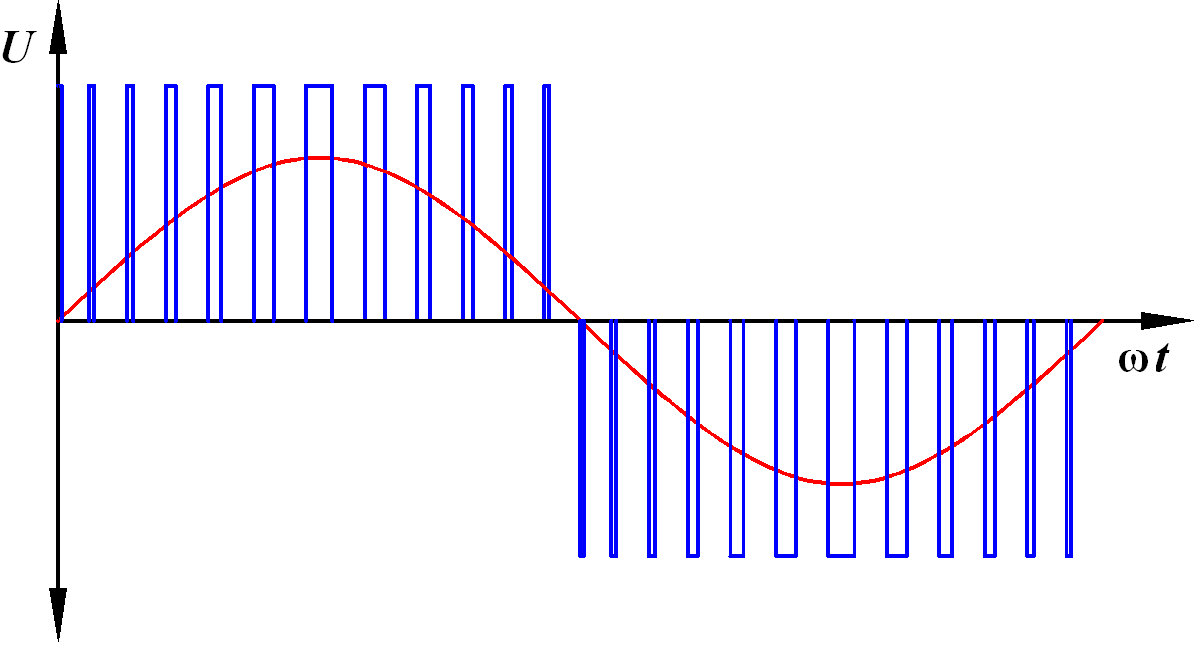
\includegraphics[width=0.45\linewidth]{images/StromBLDC} \label{figStromBLDC} 	}
\caption[BLDC Motor]{Aufbau BLDC und PWM-Ansteuerung}
\label{fig:BLDC}
\end{figure}

Angesteuert wird jede Phase über eine Halbbrücke. Die FOC-Regelungsweise (siehe Kapitel \ref{tGl_FOC}) setzt einen sinusförmigen Strom auf jeder Phase voraus, dies jeweils 120\(^\circ\) phasenverschoben. Realisiert wird dieser Strom mittels PWM-Ansteuerung der Halbbrücken. Da der Strom bei einer L-Last das Integral der Spannung ist, lässt sich ein quasi-sinusförmiger Strom generieren. Dargestellt ist dies in der Abbildung \ref{figStromBLDC}.

\begin{center}
\begin{tabular}{l|c}
\hline 
\rule[-1ex]{0pt}{2.5ex} Leerlaufstrom & 1.2A \\ 
\hline 
\rule[-1ex]{0pt}{2.5ex} Maximalstrom & 50A \\ 
\hline
\rule[-1ex]{0pt}{2.5ex} Eingangsspannung & 2..10 x 3.6 Lipo (25.2V) \\ 
\hline
\rule[-1ex]{0pt}{2.5ex} Maximale Leistung & 1815W \\ 
\hline
\rule[-1ex]{0pt}{2.5ex} Maximaler Zug & 6700g \\ 
\hline
\rule[-1ex]{0pt}{2.5ex} Nennstrom & 42.5A \\ 
\hline
\rule[-1ex]{0pt}{2.5ex} Gewicht & 460g \\ 
\hline
\rule[-1ex]{0pt}{2.5ex} Schaft & 8mm \\ 
\hline
\rule[-1ex]{0pt}{2.5ex} Abmessung & \O 50 x 65mm \\ 
\hline
\rule[-1ex]{0pt}{2.5ex} Innenwiderstand & 0.0361$\Omega$ \\ 
\hline	
\end{tabular} 
\captionof{table}{BLDC Daten}
\label{tabBLDCdaten}
\end{center}

\todo{e-Deutsch uebersetzung und Formatierung usw}


\subsection{FOC}
\label{tGl_FOC}

Für die feldorientierte Regelung werden die Phasenströme des Motors gemessen und anschliessend in ein rotorfestes Bezugssystem transformiert (\textbf{Clarke- und Park-Transformation}). Dazu wird die Rotorlage benötigt, diese wird gemessen oder berechnet (\textbf{nonlinear observer}). Im rotorfesten Bezugssystem wird das Drehmoment und die Flussdichte des Motors mit einem \textbf{PI- oder PID-Regler} geregelt. Anschliessend werden diese Werte zurücktransformiert und für die PWM-Ansteuerung des Motors genutzt(\ref{tGl_HBrugg}). \todo{verständlicher?!}

\subsubsection{Clarke- und Park-Transformation}
Das allgemeine Prinzip der Transformationen lautet:
Ein kompliziertes Problem wird in ein anderes Koordinatensystem transformiert. Das transformierte Problem ist dort viel einfacher zu lösen. Die so leicht gefundene transformierte Lösung wird rücktransformiert, wodurch die Lösung des komplizierten Problems im ursprünglichen Koordinatensystem erhalten wird. Ein mögliches Beispiel dafür ist die Laplace-Transformation von Differentialgleichungen. \todo{Luxus: Bild/Schema der Trafo von Fr. Beneduce}
\\
Das komplizierte Problem ist hier die Ansteuerung des Motors mittels einer dreiphasigen PWM. Mit der Clarke-Transformation wird in ein statorfestes Koordinatensystem gewechselt, mit der anschliessenden Park-Transformation in ein rotorfestes. Das transformierte Problem ist nun linear und mit einem einfachen PI (oder PID) -Regler lösbar. \\
Anschliessend wird die gefundene Lösung zurücktransformiert. Dabei kann die komplette Rücktransformation (inverse Park- und inverse Clarke Transformation) ausgeführt und anschliessend der Motor über eine PWM angesteuert werden, oder aber es wird nur bis ins statorfeste Koordinatensystem rücktransformiert (inverse Park Transformation), dann wird der Motor über eine Raumvektor-PWM (SVPWM) angesteuert.

\todo{ev. subsections nummeriert?!}

\begin{figure} [H]
	\centering
	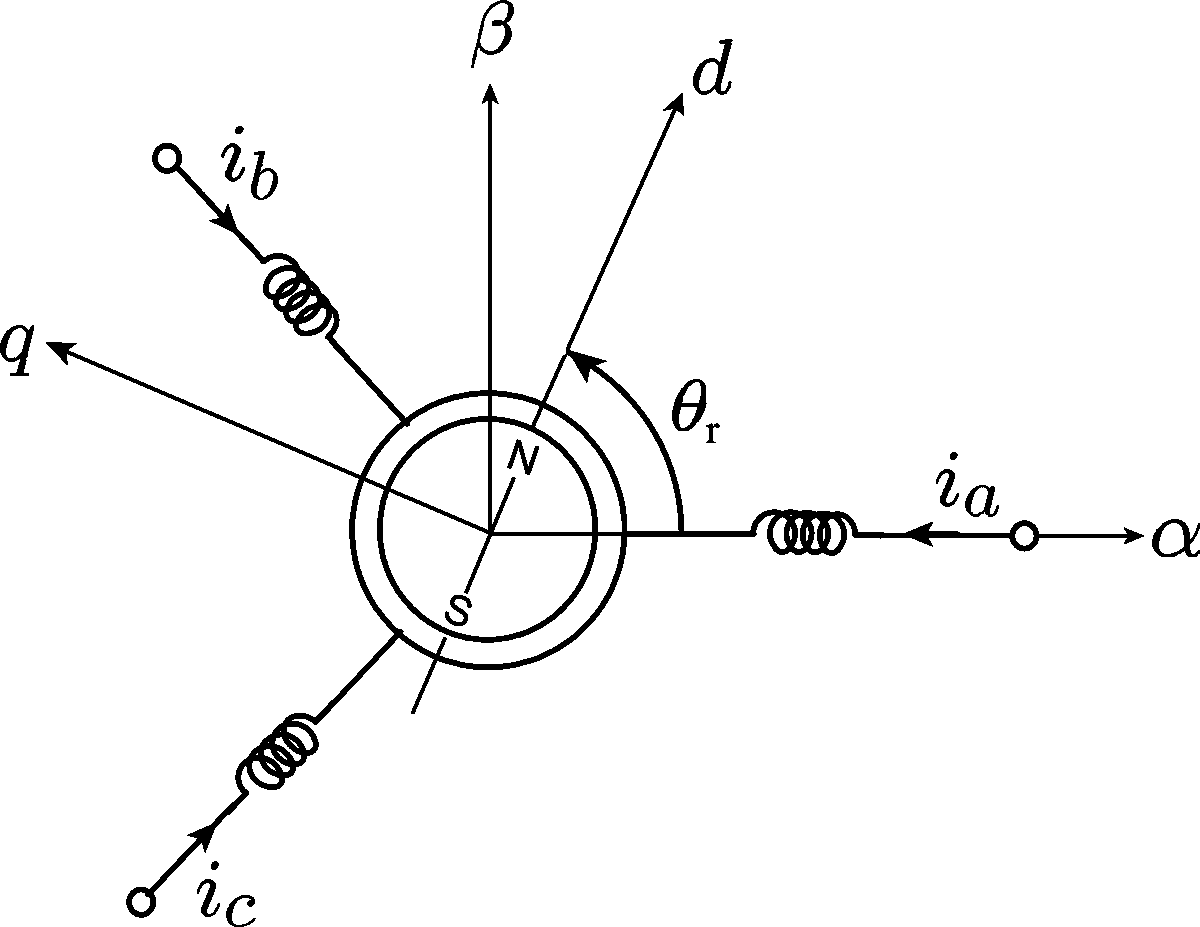
\includegraphics[width=.45\linewidth]{images/trafo_schematicPMSM}
	\caption{Schematische Darstellung einer PMSM mit den drei Koordinatensystemen \cite{IEEE_nonlinearObserver}}
	\label{fig:trafoschematicpmsm}
\end{figure} \todo{grösse des Bildes...}

\subsubsection*{Clarke-Transformation}
\todo{weitere unterstrukturierung mgl?}
Die Clarke-Transformation wechselt die mehr- bzw. dreiphasigen Grössen (z.B. Phasenströme) in ein statorfestes Bezugssystem\cite{ClarkeTrafo_Wiki}. Das kartesische Koordinatensystem ist in der komplexen Ebene. Die drei Phasenströme I$_{a}$, I$_{b}$ und I$_{c}$ werden auf zwei komplexwertige Ströme I$_{\alpha}$ und I$_{\beta}$ abgebildet. Dargestellt ist die Transformation in der Abbildung \ref{fig:trafoschematicpmsm}.
Die mathematische Formulierung lautet:
\begin{equation}\label{ClarkeTrafo}
\left[
\begin{array}{c}
I_\alpha \\ 
I_\beta
\end{array} 
\right]
= \frac{2}{3}
\left[
\begin{array}{ccc}
1 & -\frac{1}{2} & -\frac 12 \\ 
0 & \frac{\sqrt{3}}{2} & -\frac{\sqrt{3}}{2}
\end{array} 
\right] 
\left[
\begin{array}{c}
I_A \\ 
I_B \\
I_C
\end{array} 
\right]
\end{equation}
\todo{Abstände zwischen den Zeilen der Matrix?! ... schönere Darstellung gewünscht; Entscheid ob Multiplikationspunkt cdot dazwischen}
Die inverse Clarke-Transformation wird entsprechend durch folgende Gleichung beschrieben:
\begin{equation}\label{invClarkeTrafo}
\left[
\begin{array}{c}
I_A \\ 
I_B \\
I_C
\end{array} 
\right]
= 
\left[
\begin{array}{cc}
1 & 0 \\
-\frac{1}{2} & \frac{\sqrt{3}}{2} \\
-\frac 12  & -\frac{\sqrt{3}}{2}
\end{array} 
\right] 
\left[
\begin{array}{c}
I_\alpha \\ 
I_\beta
\end{array} 
\right]
\end{equation}


\subsubsection*{Park-Transformation}
Die Park-Transformation transformiert die Grössen I$_{\alpha}$ und I$_{\beta}$ in ein rotorfestes Bezugssystem\cite{leiserEffizienterBLDC}. Dieses neue kartesische Koordinatensystem besteht aus zwei Achsen. Von aussen gesehen (ruhendes Bezugssystem) rotiert es mit der gleichen Winkelgeschwindigkeit wie der Rotor. Eine Achse wird als d-Achse (direct axis) bezeichnet, die andere als q-Achse (quadrature axis). Die d-Achse beschreibt die magnetische Flussdichte des Rotors, die q-Achse das Drehmoment des Rotors. \\
Ausgehend vom statorfesten Bezugssystem benötigt es nur noch eine Rotation, um die Grössen in das rotorfeste Bezugssystem zu transformieren\cite{dqTrafo_Wiki}. Mathematisch gesehen geschieht die Transformation also über eine Drehmatrix, dargestellt ist die Transformation in der Gleichung \ref{ParkTrafo}. 
\begin{equation}\label{ParkTrafo}
\left[
\begin{array}{c}
I_d \\ 
I_q
\end{array} 
\right]
= 
\left[
\begin{array}{cc}
\cos (\theta) & \sin(\theta) \\
-\sin(\theta)  & \cos(\theta)
\end{array} 
\right] 
\left[
\begin{array}{c}
I_\alpha \\ 
I_\beta
\end{array} 
\right]
\end{equation}

Die inverse Park-Transformation wird entsprechend durch folgende Gleichung beschrieben:
\begin{equation}\label{invParkTrafo}
\left[
\begin{array}{c}	
I_\alpha \\ 
I_\beta
\end{array} 
\right]
= 
\left[
\begin{array}{cc}
\cos (\theta) & -\sin(\theta) \\
\sin(\theta)  & \cos(\theta)
\end{array} 
\right] 
\left[
\begin{array}{c}
I_d \\ 
I_q
\end{array} 
\right]
\end{equation}

\subsubsection*{d/q-Transformation} 
Die Clarke- und Park-Transformation kann auch in einem Schritt durchgeführt werden, je nach Quelle wird diese dann auch Park-Transformation oder d/q-Transformation genannt\cite{dqTrafo_Wiki}.
Die mathematische Formulierung lautet:
\begin{equation}\label{dqTrafo}
\left[
\begin{array}{c}
I_d \\ 
I_q
\end{array} 
\right]
= \frac{2}{3}
\left[
\begin{array}{ccc}
\cos (\theta) & \cos (\theta-\frac{2\pi}{3}) & \cos (\theta-\frac{4\pi}{3}) \\ 
-\sin (\theta) & -\sin (\theta-\frac{2\pi}{3}) & -\sin (\theta-\frac{4\pi}{3})
\end{array} 
\right] 
\left[
\begin{array}{c}
I_A \\ 
I_B \\
I_C
\end{array} 
\right]
\end{equation}

Die inverse d/q-Transformation lautet:
\begin{equation}\label{invdqTrafo}
\left[
\begin{array}{c}
I_A \\ 
I_B \\
I_C
\end{array} 
\right]
=
\left[
\begin{array}{cc}
\cos (\theta) & -\sin (\theta) \\
\cos (\theta-\frac{2\pi}{3}) & -\sin (\theta-\frac{2\pi}{3}) \\
\cos (\theta-\frac{4\pi}{3}) & -\sin (\theta-\frac{4\pi}{3}) 
\end{array} 
\right] 
\left[
\begin{array}{c}
I_d \\ 
I_q
\end{array} 
\right]
\end{equation}


\subsubsection{PI-Regler}
Der PI-Regler ist ein Regler mit einem Proportional- (P) und einem Integral- (I) Glied. Dies sind elementare Glieder der Regelungstechnik. Das P-Glied entspricht einer Multiplikation des Eingangs mit einer zeitunabhängigen Konstanten, das P-Glied einer Integration des Eingangs. 
\\
Die Regelung mit einem PI-Regler geschieht im rotorfesten Bezugssystem. Gegenstand der Regelung sind die Flussdichte des Motors (d-Komponente) und das Drehmoment (q-Komponente). Bei einem permanenterregten Motor ist diese Regelung vereinfacht. In der Abb.\ref{fig:trafoschematicpmsm} ist ersichtlich, dass die d-Achse in Richtung des Permanentmagneten zeigt. Das grösste resultierende Moment wird erreicht, wenn die resultierende Flussdichte im Stator um 90\(^\circ\) zur zeitlich konstanten Flussdichte des Rotors verschoben ist. Dies zeigt also genau in Richtung der q-Achse. Die resultierende Flussdichte liegt also auf der q-Achse und hat deshalb keinen d-Anteil. Der Sollwert der d-Komponente wird also null. Das Drehmoment kann somit direkt über die q-Komponente geregelt werden.

\subsubsection{Nonlinear Observer}
Die Park-Transformation benötigt die momentane Lage des Rotors. Da der vorgegebene Motor nicht über integrierte Sensoren (wie beispielsweise Hall-Sonden) verfügt, die Ansteuerung also sensorlos erfolgt, muss der Winkel der Rotorlage auf einem anderen Weg herausgefunden werden. Dazu gibt es verschiedene Varianten. 
Im Team wurde entschieden, die Winkelschätzung über einen nichtlinearen Beobachter, nonlinear observer genannt, vorzunehmen. Dazu wird ein mathematisches Modell des Motors erstellt. Zudem werden die Phasenströme gemessen. Mit diesen Informationen wird eine Simulation des Motors durchgeführt, und aufgrund der aktuellen Parameter wird die Position ermittelt. Dies funktioniert, weil von den Phasenströme auf die Lage des Motors geschlossen werden kann. Beschrieben wird dieses Verfahren in \cite{IEEE_nonlinearObserver}. Grundsätzlich wird in diesem Verfahren folgende Zustandsvariable definiert:

\begin{equation}\label{statevar}
	x = Li_{\alpha\beta}+\psi_m \left[ \begin{array}{c} cos\theta \\ sin\theta \end{array} \right]
\end{equation}

Der nichtlineare Beobachter wird nun um die in \ref{statevar} definierte Zustandsvariable erstellt:
\begin{equation}\label{nonlinobs}
	\dot{\hat{x}} = y + \frac{\lambda}{2}\eta(\hat{x})[\psi_m^2-||\eta(\hat{x})||^2]
\end{equation}

Grundsätzlich werden nun periodisch die Ströme gemessen, clarke-transformiert und der Observer ausgeführt. Der Observer braucht dafür sehr exakte Kennzahlen des Motors wie Motorkonstante, Seriewiderstand und Induktivität. So kann der Winkel $\hat{\theta}$ geschätzt werden. Die Berechnungen sind auf dem gewählten Mikrocontroller dank FPU schnell ausgeführt.

\subsection{H-Brücke}
\label{tGl_HBrugg}
Wie in Abbildung \ref{fig:BLDC} auf Seite \pageref{fig:BLDC} zu sehen ist, muss am Motor eine sinusförmige Spannung anliegen. Die FOC-Berechnungen aus Kapitel \ref{tGl_FOC} ergeben zeitdiskrete Spannungswerte. Diese werden mit der Raumvektor-PWM Methode in PWM Signale umgewandelt die mit der H-Brücke ausgegeben werden. Die H-Brücke besteht aus drei Halbbrücken mit je zwei N-Kanal MOSFETs. 
\begin{center}
	\begin{circuitikz}[scale=2]
		\draw[color=black]
		% Fet, Fet and Resistor
		(0,1) node[nigfete] (nmos1) {}
		(0,0) node[nigfete] (nmos2) {}
		(nmos1.S) to (nmos2.D)
		(nmos2.S) to [R, l_=$R_{sense1}$] (0,-1.5) -- (1,-1.5)
		(nmos1.D) |- (1,1.5)
		% Fet, Fet and Resistor
		(2,1) node[nigfete] (nmos3) {}
		(2,0) node[nigfete] (nmos4) {}
		(nmos3.S) to (nmos4.D)
		(nmos4.S) to [R, l_=$R_{sense2}$] (2,-1.5) -- (2,-1.5)
		(nmos3.D) |- (1,1.5)
		% Fet, Fet
		(4,1) node[nigfete] (nmos5) {}
		(4,0) node[nigfete] (nmos6) {}
		(nmos5.S) to (nmos6.D)
		(nmos6.S) |- (1,-1.5)
		(nmos6.D) |- (1,1.5)

		% ground
		(2,-1.5) node[ground]{}
		% supply
		(2,1.5) to [short,-o] (2,2) node[right]{$V_{BAT}$}
		% gates
		(nmos1.G) to [short,-o] ++(-0.1,0) node[left]{$AH$}
		(nmos2.G) to [short,-o] ++(-0.1,0) node[left]{$AL$}
		(nmos3.G) to [short,-o] ++(-0.1,0) node[left]{$BH$}
		(nmos4.G) to [short,-o] ++(-0.1,0) node[left]{$BL$}
		(nmos5.G) to [short,-o] ++(-0.1,0) node[left]{$CH$}
		(nmos6.G) to [short,-o] ++(-0.1,0) node[left]{$CL$}
		%outputs
		(nmos1.S) ++(0,-0.1) to [short,-o] ++(0.5,0) node[right]{$A$}
		(nmos3.S) ++(0,-0.1) to [short,-o] ++(0.5,0) node[right]{$B$}
		(nmos5.S) ++(0,-0.1) to [short,-o] ++(0.5,0) node[right]{$C$}
		;
		% junctions
		\fill (2,-1.5) circle(1pt);
		\fill (2,1.5) circle(1pt);
		\fill (nmos1.S) ++(0,-0.1) circle(1pt);
		\fill (nmos3.S) ++(0,-0.1) circle(1pt);
		\fill (nmos5.S) ++(0,-0.1) circle(1pt);
	\end{circuitikz}
	\captionof{figure}{H-Brücke zur Motoransteuerung}
	\label{fig:hbridge}
\end{center}

Mit den sogenannten High-Side MOSFETs kann jede Phase einzeln auf die Batteriespannung geschaltet werden. Die Low-Side FETs arbeiten symmetrisch dazu und können die Phase auf Batteriemasse schalten. Durch die berechneten PWM kann so ein dreiphasiger Sinus approximiert werden. 

Damit nicht gleichzeitig die High- und Low-Side FETs einer Phase eingeschaltet sind, was zu einem Kurzschluss führen würde, ist im Treiber IC eine Totzeit-Schaltung eingebaut. Wird der eine FET ausgeschaltet, sind für eine kurze Zeit beide ausgeschaltet, bevor der nächste eingeschaltet werden kann. Dieses Verfahren wird \todo{Deadtime? Davor: Dedatime}Deadtime genannt.

\subsection{Funkübertragung}
Die Funkübertragung wird mit einem RFM75-Modul ermöglicht. Dieses kommuniziert auf 2.4GHz in einem extrem einfachen proprietären Protokoll. Für dieses Projekt wurde der erste von 83 möglichen Datenkanälen genutzt. Die genaue Übertragungsfrequenz ist somit 2,401GHz. Die folgende Tabelle wurde sinngemäss aus dem Datenblatt des Funkmoduls übernommen und zeigt den Aufbau der übermittelten Pakete, wie sie für dieses Projekt aus den Einstellungen des Moduls gesendet werden.
\begin{center}
	\begin{tabularx}{0.3\textwidth}{l|c}
		Inhalt & Grösse \\ \hline
		Preample& 1 Bit \\ \hline
		Adresse &3 Byte \\ \hline
		Payload Länge& 6 Bit \\ \hline
		Paket-ID &2 Bit \\ \hline
		NO ACK & 1 Bit \\ \hline
		Daten & 1 Byte \\ \hline
		CRC & 1 Byte \\ \hline
	\end{tabularx}
	\captionof{table}{Paketaufbau des Funkmoduls}
\end{center}

Das Modul sendet im Stromsparmodus mit einer Datenrate von maximal 1Msps was für eine angestrebte Übertragungsrate von 100 8-Bit-Werten pro Sekunde ausreicht.
\label{tGl_RF}
